\begin{frame}{A árvore de recursão}
    \metroset{block=fill}

    Analisemos a árvore de recursão da função $f$ para $n = 4$.

    \begin{center}
        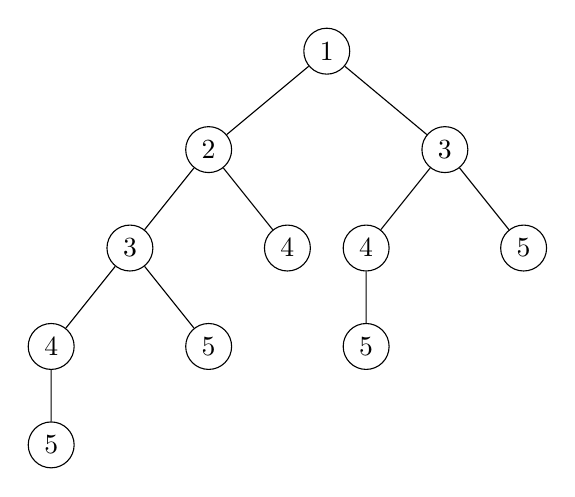
\begin{tikzpicture}[every node/.style={circle,inner sep=3pt,draw},level 1/.style={sibling distance=3cm},level 2/.style={sibling distance=2cm},level distance=1.25cm]
            \node {1} 
            child {
                node {2}
                child {
                    node {3}
                    child {
                        node {4}
                        child {node {5}}
                    }
                    child {node {5}}
                }
                child {
                    node {4}
                }
            }
            child {
                node {3}
                child {
                    node {4}
                    child {node {5}}
                }
                child {node {5}}
            };
        \end{tikzpicture}
    \end{center}

    Temos repetidas chamadas recursivas para $i = 3, 4, 5$. Porém, memoizando a resposta de $f(i)$ para cada $i$, precisamos chamar $f(i)$ uma vez para cada valor de $i$ diferente, tornando a solução $O(n)$.

\end{frame}
